% This is LLNCS.DEM the demonstration file of
% the LaTeX macro package from Springer-Verlag
% for Lecture Notes in Computer Science,
% version 2.3 for LaTeX2e
%
\documentclass{llncs}
%
\usepackage{makeidx}  % allows for indexgeneration
\usepackage[utf8]{inputenc}
\usepackage[english]{babel}
\usepackage{indentfirst}
\usepackage{graphicx}
\usepackage{subfig}
%
\begin{document}

\mainmatter              % start of the contributions
%
\title{Text Mining Wikipedia\\to extract historical facts}
%
\titlerunning{Text Mining Wikipedia\\to extract historical facts}  % abbreviated title (for running head)
%                                     also used for the TOC unless
%                                     \toctitle is used
%
\author{João Valente \and João Gradim}
%
\authorrunning{João Valente, João Gradim}   % abbreviated author list (for running head)
%
%%%% list of authors for the TOC (use if author list has to be modified)
\tocauthor{João Valente, João Gradim}
%
\institute{Faculdade de Engenharia da Universidade do Porto,\\
Rua do Dr. Roberto Frias, s/n, Porto, Portugal}

\maketitle              % typeset the title of the contribution

\begin{abstract}
The abstract should summarize the contents of the paper
using at least 70 and at most 150 words. It will be set in 9-point
font size and be inset 1.0 cm from the right and left margins.
There will be two blank lines before and after the Abstract. \dots
\end{abstract}

\section{Problem}

\section{Objectives}

\begin{itemize}
	\item To provide an easily queryable database of historical events of major importance
	\item To allow users to use natural language to perform queries
	\item To be able to cross-reference historical events and link figures, places
	\item To be able to group events in categories to further refine search
\end{itemize}

\section{Motivation}

Younger population knows progressively less and less about history and human achievements. A simple interface would provide a means to an easy access to information and could boost interest in learning.\\

\section{State of the Art}

\subsection{Natural Language Processing and Tokenization}

\begin{itemize}
	\item The Stanford Parser
\end{itemize}

\subsection{HTML Parsing (Ruby)}

\begin{itemize}
	\item HPricot
	\item Nokogiri
\end{itemize}

\subsection{Classification and Machine Learning (Ruby)}

\begin{itemize}
	\item Naïve Bayes Classification
	\begin{itemize}
		\item Bayesian Networks
	\end{itemize}
\end{itemize}

\section{Text Extraction}

\section{Text classification}

\section{Natural Language Processing}

\subsection{People Extraction}

\begin{figure}[h]
	\centering
	\includegraphics[width=40mm]{dia/people.eps}
	\caption{Subtree relating to proper nouns, from where names of people involved can be extracted}
	\label{fig:people_extraction}
\end{figure}

\newpage
\subsection{Local extraction}

\begin{figure}[h]
	\centering
	\subfloat[Local extraction pattern 1]{\label{fig:local_1}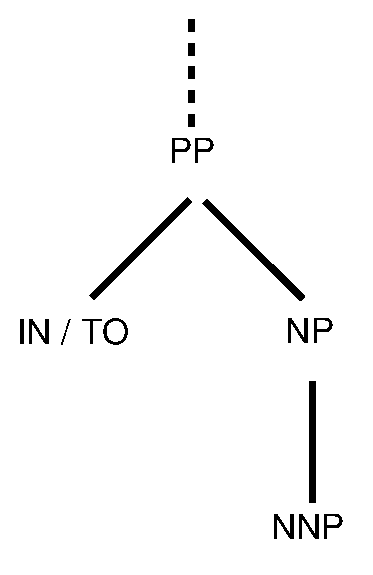
\includegraphics[width=0.35\textwidth]{dia/local_1.eps}}     
	\hspace{20mm}
	\subfloat[Local extraction pattern 2]{\label{fig:local_2}\includegraphics[width=0.45\textwidth]{dia/local_2.eps}}
	\caption{Subtrees for event location extraction}
	\label{fig:locals}
\end{figure}

This kind of structure is present on most events parsed from Wikipedia and allows the retrieval of the phisical location of the occurence, mainly the country or a city in a determined country.

%
\section{Main implementation problems}

Wikipedia is an open knowledge base, relying mainly on user generated content. As such, it's difficult to ensure a proper and constant textual structure for information. Although the pages for the most recent centuries (aprox. 18th century) have a well defined an constant HTML strutcture that allows for reliable information retrieval, there are many years that don't follow this structure, leading to specific parsing cases.\\
\ \\
This openness lead to another problem: an HTML structure not suited for easy parsing. A series of workarounds had to be implemented to successfuly extract useful information.

\newpage
%
% ---- Bibliography ----
%
\begin{thebibliography}{}
%
\bibitem[1990]{santorini}
Santorini, B. :
Part-of-Speech Tagging Guidelines for the
Penn Treebank Project (3rd Revision, 2nd Printing).
(July 1990)

\bibitem[1995]{bies}
Bies, A., Ferguson, M., Katz, K., MacIntyre, R. :
Bracketing Guidelines for Treebank II
Penn Treebank Project
(June 1995)

\end{thebibliography}
\clearpage
\addtocmark[2]{Author Index} % additional numbered TOC entry
\renewcommand{\indexname}{Author Index}
\printindex
\clearpage
\addtocmark[2]{Subject Index} % additional numbered TOC entry
\markboth{Subject Index}{Subject Index}
\renewcommand{\indexname}{Subject Index}
\input{subjidx.ind}
\end{document}
